\documentclass{article}\usepackage[]{graphicx}\usepackage[]{color}
%% maxwidth is the original width if it is less than linewidth
%% otherwise use linewidth (to make sure the graphics do not exceed the margin)
\makeatletter
\def\maxwidth{ %
  \ifdim\Gin@nat@width>\linewidth
    \linewidth
  \else
    \Gin@nat@width
  \fi
}
\makeatother

\definecolor{fgcolor}{rgb}{0.345, 0.345, 0.345}
\newcommand{\hlnum}[1]{\textcolor[rgb]{0.686,0.059,0.569}{#1}}%
\newcommand{\hlstr}[1]{\textcolor[rgb]{0.192,0.494,0.8}{#1}}%
\newcommand{\hlcom}[1]{\textcolor[rgb]{0.678,0.584,0.686}{\textit{#1}}}%
\newcommand{\hlopt}[1]{\textcolor[rgb]{0,0,0}{#1}}%
\newcommand{\hlstd}[1]{\textcolor[rgb]{0.345,0.345,0.345}{#1}}%
\newcommand{\hlkwa}[1]{\textcolor[rgb]{0.161,0.373,0.58}{\textbf{#1}}}%
\newcommand{\hlkwb}[1]{\textcolor[rgb]{0.69,0.353,0.396}{#1}}%
\newcommand{\hlkwc}[1]{\textcolor[rgb]{0.333,0.667,0.333}{#1}}%
\newcommand{\hlkwd}[1]{\textcolor[rgb]{0.737,0.353,0.396}{\textbf{#1}}}%
\let\hlipl\hlkwb

\usepackage{framed}
\makeatletter
\newenvironment{kframe}{%
 \def\at@end@of@kframe{}%
 \ifinner\ifhmode%
  \def\at@end@of@kframe{\end{minipage}}%
  \begin{minipage}{\columnwidth}%
 \fi\fi%
 \def\FrameCommand##1{\hskip\@totalleftmargin \hskip-\fboxsep
 \colorbox{shadecolor}{##1}\hskip-\fboxsep
     % There is no \\@totalrightmargin, so:
     \hskip-\linewidth \hskip-\@totalleftmargin \hskip\columnwidth}%
 \MakeFramed {\advance\hsize-\width
   \@totalleftmargin\z@ \linewidth\hsize
   \@setminipage}}%
 {\par\unskip\endMakeFramed%
 \at@end@of@kframe}
\makeatother

\definecolor{shadecolor}{rgb}{.97, .97, .97}
\definecolor{messagecolor}{rgb}{0, 0, 0}
\definecolor{warningcolor}{rgb}{1, 0, 1}
\definecolor{errorcolor}{rgb}{1, 0, 0}
\newenvironment{knitrout}{}{} % an empty environment to be redefined in TeX

\usepackage{alltt}
\usepackage{natbib}
\IfFileExists{upquote.sty}{\usepackage{upquote}}{}
\begin{document}



\title{The Adcentures of Sherlock Holmes}
\author{Akhilesh Atluri}
\maketitle

\begin{abstract}

In this Article we are building wordcloud of the words from sherlock Holmes using sherlock Holmes clip art

\end{abstract}

\textit{The Adventures of Sherlock Holmes}is a novel by SIR ARTHUR CONAN DOYLE

\section{Getting the data and getting required packages}

\begin{knitrout}
\definecolor{shadecolor}{rgb}{0.969, 0.969, 0.969}\color{fgcolor}\begin{kframe}
\begin{alltt}
\hlkwd{library}\hlstd{(dplyr)}
\hlkwd{library}\hlstd{(tidytext)}
\hlkwd{library}\hlstd{(stringr)}
\hlkwd{library}\hlstd{(wordcloud)}
\hlkwd{library}\hlstd{(tm)}
\hlkwd{library}\hlstd{(gutenbergr)}
\hlkwd{library}\hlstd{(knitr)}
\hlkwd{library}\hlstd{(wordcloud2)}

\hlcom{#After installing and bringing in all the packages let's bring in text for 'The Adventures of Sherlock Holmes'}

\hlkwd{gutenberg_works}\hlstd{(}\hlkwd{str_detect}\hlstd{(title,}\hlstr{'The Adventure'}\hlstd{))}
\end{alltt}
\begin{verbatim}
## # A tibble: 171 x 8
##    gutenberg_id
##           <int>
##  1           74
##  2          500
##  3          909
##  4         1194
##  5         1218
##  6         1372
##  7         1644
##  8         1661
##  9         1825
## 10         2343
## # ... with 161 more rows, and 7 more variables: title <chr>, author <chr>,
## #   gutenberg_author_id <int>, language <chr>, gutenberg_bookshelf <chr>,
## #   rights <chr>, has_text <lgl>
\end{verbatim}
\begin{alltt}
\hlstd{sherlock}\hlkwb{<-}\hlkwd{gutenberg_download}\hlstd{(}\hlnum{1661}\hlstd{)}
\end{alltt}
\end{kframe}
\end{knitrout}

\section{Getting the words}
Now using dplyr lets get words without blank lines

\begin{knitrout}
\definecolor{shadecolor}{rgb}{0.969, 0.969, 0.969}\color{fgcolor}\begin{kframe}
\begin{alltt}
\hlstd{sherlock_words}\hlkwb{<-}\hlstd{sherlock}\hlopt
  \hlkwd{unnest_tokens}\hlstd{(word,text)}
\end{alltt}
\end{kframe}
\end{knitrout}

\noindent Let's get rid of all the unwanted words such as 'the' ,'and' etc..

\begin{knitrout}
\definecolor{shadecolor}{rgb}{0.969, 0.969, 0.969}\color{fgcolor}\begin{kframe}
\begin{alltt}
\hlstd{sherlock_words}\hlkwb{<-}\hlstd{sherlock_words}\hlopt
  \hlkwd{filter}\hlstd{(}\hlopt{!}\hlstd{(word} \hlopt \hlstd{stop_words}\hlopt{$}\hlstd{word))}
\end{alltt}
\end{kframe}
\end{knitrout}

\noindent Now let's group each word and get the count of each word
\begin{knitrout}
\definecolor{shadecolor}{rgb}{0.969, 0.969, 0.969}\color{fgcolor}\begin{kframe}
\begin{alltt}
\hlstd{sherlock_freq}\hlkwb{<-}\hlstd{sherlock_words}\hlopt
  \hlkwd{group_by}\hlstd{(word)}\hlopt
  \hlkwd{summarize}\hlstd{(}\hlkwc{count}\hlstd{=}\hlkwd{n}\hlstd{())}
\end{alltt}
\end{kframe}
\end{knitrout}


\section{wordcloud2}

\begin{knitrout}
\definecolor{shadecolor}{rgb}{0.969, 0.969, 0.969}\color{fgcolor}\begin{kframe}
\begin{alltt}
\hlkwd{wordcloud}\hlstd{(sherlock_freq}\hlopt{$}\hlstd{word,sherlock_freq}\hlopt{$}\hlstd{count,}\hlkwc{min.freq} \hlstd{=} \hlnum{25}\hlstd{)}
\end{alltt}
\end{kframe}
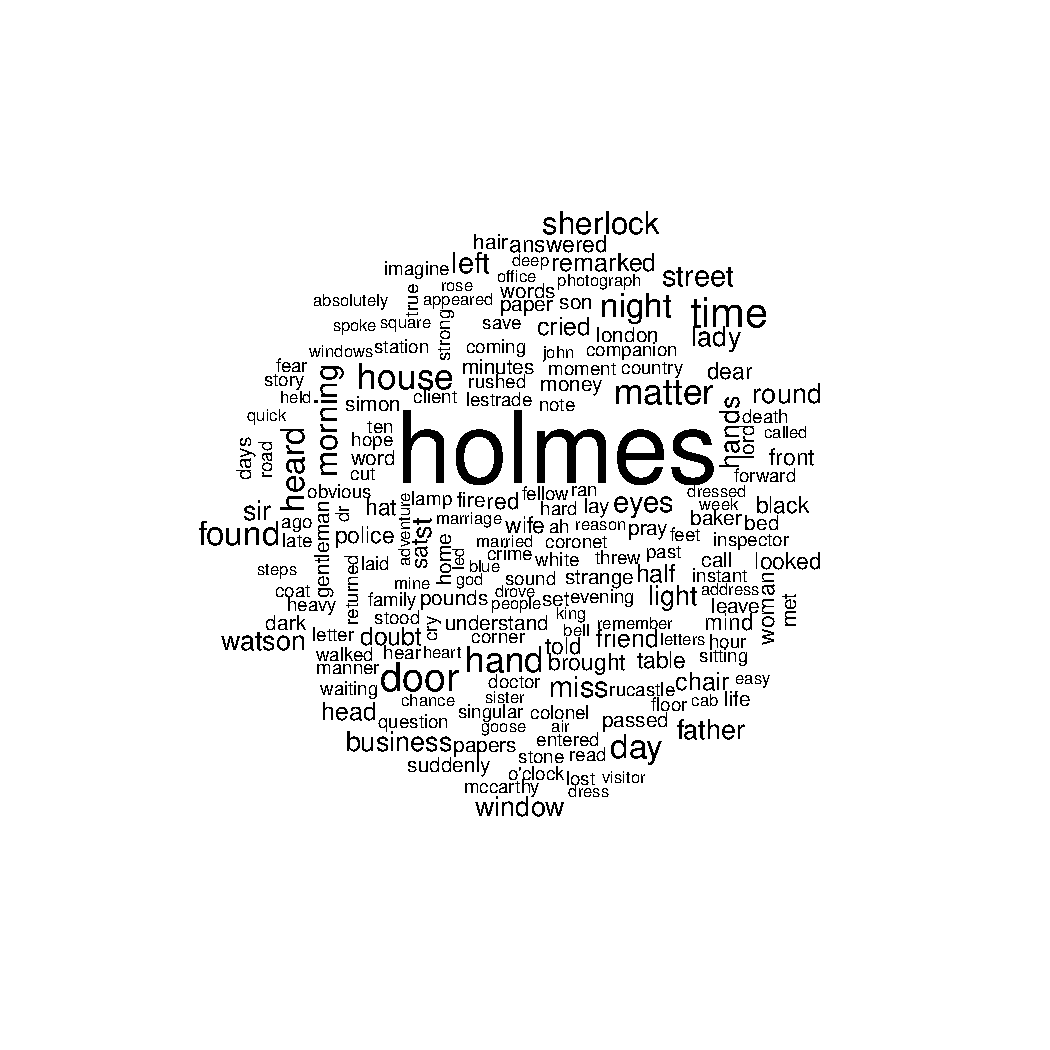
\includegraphics[width=\maxwidth]{figure/unnamed-chunk-5-1} 

\end{knitrout}



\bibliographystyle{apa}
\bibliography{article}
\nocite{*}

\end{document}
